%! TEX root = /Users/manunavjeevan/Documents/UCLA/Third Year/Reading Group/wcep.tex

\subsection{Covering Numbers}%
\label{subsec:covering}

This section roughly covers section 2.6 in Van Der Vaart and Wellner.

Recall that for the covering Donsker Theorem, Theorem~\ref{thm:vdv2.5.2}, we require the uniform entropy bound:
\[
	\int_{0}^{\infty}  \sup_{Q\in\calQ} \sqrt{\log \calN\left(\eps\|F\|_{Q,2},\calF,L_2(Q)\right)}\;d\eps < \infty\tag{UEB}\label{eq:uniform-entropy-bound-2}
.\] 
where the supremum under the integral is taken over the set of all finitely discrete probability measures \(\calQ\). If we can show that \(\calF\) is such that \(\sup_\calQ \log \calN\left(\eps\|F\|_{Q,2},\calF,L_2(Q)\right) \lesssim \left(\frac{1}{\eps}\right)^{2+\delta}\) for some \(\delta > 0\) then we are fine as this will integrate to a finite number.

\subsubsection{VC Classes of Sets}%
\label{subsubsec:vc-class}

A typical way to show that a class of sets \(\calF\) satisfies the \eqref{eq:uniform-entropy-bound} will be to show that it has a limited ``VC-Dimension'', where ``VC'' stands for Vapnick and Cervonenkis. What does this mean?

Let \(\calC\) be a collection of subsets of some set \(\calX\), that is \(\calC \subseteq 2^\calX\). An arbitrary set of points \(\{x_1,\dots,x_n\}\) possesses \(2^n\) subsets.

\begin{definition}[Picking Out]
	\label{def:picks-out}
	Let \(A \subset \{x_1,\dots,x_n\}\). The collection \(\calC\) picks out \(A\) if \(A = C \cap \{x_1,\dots,x_n\}\) for some \(C \in\calC\). We define the number of subsets of \(\{x_1,\dots,x_n\}\) picked out by \(\calC\) as 
	\begin{equation}
		\label{eq:delta-n}
		\Delta_n(\calC,x_1,\dots,x_n) = \#\left\{C\cap\{x_1,\dots,x_n\}:C\in\calC \right\}	
	\end{equation}
\end{definition}

\begin{definition}[Shattering]
	\label{def:shattering}
	A collection \(\calC\) shatters \(\{x_1\dots,x_n\}\) if it can pick out all of its \(2^n\) subsets.
\end{definition}

\begin{definition}[VC Index]
	\label{def:vc-index}
	The VC-Index, \(V(\calC)\) is the smallest \(n\in\SN\) such that \emph{no} set of size \(n\) is shattered by \(\calC\). Equivalently
	\begin{equation}
		\label{eq:vc-index}
		V(\calC) = \inf\left\{n : \max_{x_1,\dots,x_n} \Delta_n(\calC,x_1,\dots,x_n)<2^n\right\}
	\end{equation}
\end{definition}

\begin{definition}[VC Class]
	\label{def:vc-class}
	A collection \(\calC\) of measurable sets is called VC Class if  \(V(\calC)<\infty\). 
\end{definition} 

\begin{remark*}
	Notice that in the Definition of the VC Index, we require that \textit{no} set of size \(n\) is shattered by \(\calC\) rather than requiring that \(n\) be the smallest number such that there exits \textit{any} set of size \(n\) that is not shattered by \(\calC\).
\end{remark*}

\begin{example*}
	\label{ex:vc-indices}
	Suppose \(\calC = \left\{(-\infty,c]:\text{for some }c\in\SR\right\}\). Then any set \(\{x_1\}\) has subsets \(\emptyset\) and \(\{x_1\}.\) For \(\emptyset\) we have that \(\emptyset \subset (-\infty,c]\cap \{x_1\} \) for any \(c < x_1\) while for \(\{x_1\}\) we have that \(\{x_1\}\subseteq (-\infty,c]\cap\{x_1\} \) for any \(c \geq x_1\). Thus we have that \(\calC\) shatters any single element subset of \(\SR\).

	However, take a two element subset \(\{x_1,x_2\}\subset \SR\). Without loss of generality take \(x_1 < x_2\). There are four subsets to consider, \(\emptyset, \{x_1\},\{x_2\},\{x_1,x_2\}\). We can see that there is no set \(C \in \calC\) such that \(C \cap \{x_1,x_2\} = \{x_2\}\), if we take \(C = (\infty,c]\) for some \(c < x_2\) we get that \(C \cap \{x_1,x_2\} = \{x_1\}\) whereas if we take \(C = (-\infty, c]\) for some \(c \geq x_2\) we get that \(C\cap\{x_1,x_2\} = \{x_1,x_2\}\). This exhausts all sets in \(\calC\). 

	Since \(\{x_1,x_2\}\) is arbitrary, we can conclude that the VC Index of \(\calC\) is two, \(V(\calC)=2\).
\end{example*}

\begin{example*}
	\label{ex:vc-indices-2}
	Let \(\calC_1 = \left\{(a,b]:a<b\text{ for } a,b \in \SR\right\}\). Note that this collection is larger than the collection. Now however, given a set \(\{x_1,x_2\} \) with \(x_1 < x_2\) we can pick out \(\{x_2\}\) with the set \((x_1,x_2]\in\calC_1\).

	However, now consider a three element subset \(\{x_1,x_2,x_3\}\). Without loss of generality suppose \(x_1 < x_2 < x_3\). We will try to pick out the set \(\{x_1,x_3\}\). Consider any set \(C\in \calC_1\) such that \(\{x_1,x_3\}\subset C \), a necessary condition for \(\{x_1,x_2\} = C \cap \{x_1,x_2,x_3\}\). The set \(C\) is of the form \((a,b]\) for some \(a < x_1\) and \(b \geq x_3\). However, this means that \(x_2 \in C\). So, we cannot pick out \(\{x_1,x_3\} \) with \(\calC_1\). 

	Since we can pick out one and two element subsets of \(\SR\) with \(\calC_1\), but not arbitrary three element subsets, we get that \(V\left(\calC_1\right)=3\).
\end{example*}


\begin{lemma}[Lemma 2.6.2 VdV\&W]
	\label{lemma:vdv2.6.2}
	Let \(\{x_1,\dots,x_n\}\) be arbitrary points in \(\calX\) and \(\calC\) some collection of subsets of \(\calX\). Then the total number of subsets picked out by \(\calC\), \(\Delta_n(\calC,x_1,\dots,x_n)\) picked out by \(\calC\) is bounded above by the total number of subsets of \(\{x_1,\dots,x_n\}\) shattered by \(\calC\).
\end{lemma}
\begin{proof}
	Without loss of generality assume that every \(C \in\calC\) is a subset of the given set of points so that \(\Delta_n(\calC,x_1,\dots,x_n)\) is the cardinality of \(\calC\).

	Call the class \(\calC\) \textit{hereditary} if it is closed under subsetting. That is \(C\in\calC\) and \(B \subset C\implies B \in\calC\). Each of the sets in a hereditary collection of sets is shattered\footnote{For any \(B \subset C\), \(B \in\calC\) and \(B \cap C = B\).} so that a hereditary collection shatters at least \(|\calC|\) sets and the assertion of the lemma is certainly true for hereditary collections.\footnote{Taking a look at \eqref{eq:delta-n} we see that all sets picked out by \(\calC\) are all subsets of elements of \(\calC\). Since all subsets of elements of \(\calC\) are also elements of \(\calC\), the number of sets picked out by \(\calC\) is bounded by the number of sets in \(\calC\). Every element of \(\calC\) is clearly shattered by \(\calC\) which gives the statement.} The goal now will be to show that an arbitrary collection \(\calC\) can be transformed into a hereditary collection
	without changing its cardinality or increasing the number of shattered sets.

	Given \(1 \leq i \leq n\) and \(C\in\calC\) define the set
	\[
		T_i(C) 
		= \begin{cases}
		C\setminus\{x_i\}  & \text{if } C\setminus\{x_i\}\notin\calC \\
		C &\text{otherwise }
		\end{cases}
	\]
	The map \(T_i(x)\) is injective (one-to-one) so the collections \(\calC\) and \(T_i(\calC) = \{T_i(C), C \in\calC\} \) have the same cardinalities.\footnote{Recall that \(\Delta_n(\calC,x_1,\dots,x_n) = |\calC|\) since by assumption (without loss of generality) every \(C\in\calC\) is a subset of the given set of points. This holds as well for \(T_i(\calC)\)} Furthermore, every subset \(A\subset \{x_1,\dots,x_n\}\) that is shattered by \(T_i(\calC)\) is shattered by \(\calC\). To see this note that if \(x_i\not\in A\) then \(\{\calC\cap A\} = \{T_i(\calC) \cap A\}\). Conversely if \(x_i\in A\) and \(A\) is shattered by \(T_i(\calC)\) then for every \(B\subset A\) there is a \(C\in\calC\) with \(B \cup \{x_i\} = T_i(C)\cap A\).\footnote{This is just because \(B\cup\{X_i\}\subset A\) and \(A\) is shattered by \(T_i(\calC\)} This implies that \(x_i\in T_i(C)\) so that \(T_i(C)=C\). This in turns gives that \(C\setminus\{x_i\}\in\calC\) since otherwise \(T_i\) would not have a fixed point at \(C\). Thus both \(B\cup\{x_i\}\) and \(B\setminus\{x_i\} = (C\setminus\{x_i\}) \cap A\) are picked out by \(\calC\). One of these sets equals \(B\).
	
	So the assertion of the lemma is true for \(\calC\) if it is true for \(T_i(\calC)\). Furthermore the assertion of the lemma is true for \(\calC\) if it is true for \(T(\calC)\) where \(T = T_1\circ T_2 \circ \dots\circ T_n\); by repeatedly applying the argument above we have that if a set is shattered by \(T(\calC)\) it is shattered by \(\calC\). Apply \(T\) repeatedly until the collection of sets does not change anymore. This happens after at most \(\sum_{C\in\calC}|C|\) steps (finite) since \(\sum_{C\in\calC} |T_i(C)| < \sum_{C\in\calC} |C|\) whenever the collections \(T_i(\calC)\) and \(\calC\) are different\footnote{We can think of repeatedly applying \(T\) as ``pruning'' the collection \(\calC\), removing elements from sets whose subsets are not contained in \(\calC\).}.  The collection \(\calD\) obtained in this manner has the property that \(D\setminus\{x_i\}\in\calD\) for every
	\(D\in\calD\) and every \(x_i\). So \(\calD\) is hereditary.
\end{proof}

\begin{corollary}[Corollary 2.6.3 VdV\&W]
    \label{corr:vdv2.6.3}
	For a VC-class of sets of index \(V(\calC)\) one has
	\[
		\max_{x_1,\dots,x_n} \Delta_n(\calC,x_1,\dots,x_n) \leq \sum_{j=0}^{V(\calC)-1} \binom{n}{j}
	.\]
	Consequently, the numbers on the left hand side grow polynomially of order at most \(O\left(n^{V(\calC)-1}\right)\) as \(n\to\infty\).
\end{corollary}
\begin{proof}
	The RHS of the corrolary above is the number of subsets of size at most \(V(\calC)-1\). A VC-class shatters no set of \(V(\calC)\) points. All shattered sets are of size at most \(V(\calC)-1\). The number of shattered sets gives an upper bound on \(\Delta_n\) by Lemma~\ref{lemma:vdv2.6.2}. 
\end{proof}

\begin{theorem}[Theorem 2.6.4 VdV\&W]
	\label{thm:vdv2.6.4}
	There exists a universal constant \(K\) such that, for any VC-class \(\calC\) of sets, any probability measure \(Q\), any \(r \geq 1\) and \(0 < \eps < 1\),
	\begin{equation}
		\label{eq:vdv2.6.4}
		\calN(\eps,\calC,L_r(Q)) \leq KV(\calC)(4e)^{V(\calC)}\left(\frac{1}{\eps} \right)^{rV(C)-1}
	\end{equation} 
\end{theorem}
\begin{proof}
	The proof of this Theorem takes some 3 pages in VanDerVaart so I am leaving it for now. It can be found on pages 137-139. 
\end{proof}

\begin{remark*}
	For practical purposes, if \(\calG\) is a VC-class with \(V(\calG) \geq 3\), then \(\sup_{Q\in\calQ}\calN(\eps,\calG,L_2(Q)) \lesssim \left(\frac{1}{\eps}\right)^{2+ \delta}\) which will mean that the \eqref{eq:uniform-entropy-bound} is satisfied. 
\end{remark*}

\begin{example*}
	Suppose \(\calG\) is a VC-class, that is the functions \(\mathds{1}_G\) are measurable for \(G \in \calG\) and \(V(\calG) <\infty\). Since this set of indicator functions is bounded by 1, this class is clearly Donsker. In the example above, we showed that the set \(\calG = \{(a,b]: a< b, a,d \in \SR\}\) has VC-index, \(V(\calG) = 3 < \infty\). By Theorem~\ref{thm:vdv2.6.4} (and subsequently Theorem~\ref{thm:vdv2.5.2}), this is a Donsker class. That is uniformly over \(a,b\in\SR\):
	\[
		\frac{1}{\sqrt{n}}\sum_{i=1}^n \left\{\mathds{1}[a < X_i \leq b_i] - P(a < X_i < b_i)\right\} \wcov \mathbb{G}
	.\] 
	for some tight element \(\mathbb{G}\) on \(\ell^\infty(\calG)\).
\end{example*}

All together, this is interesting for showing that collections of indicator functions are Donsker, but what about arbitrary classes of functions?

\subsubsection{VC Classes of Functions}

\begin{definition}[Subgraph]
	\label{def:subgraph}
	The subgraph of a function \(f:\calX\to\SR\) is the subset of \(\calX\times\SR\) given by 
	\[
		\left\{(x,t): t< f(x)\right\}
	.\] 
\end{definition}
\begin{remark*}
	Note that the subgraph does not include the points \(\{(x,y): y=f(x)\} \)
\end{remark*}
\begin{figure}[htpb]
	\centering
	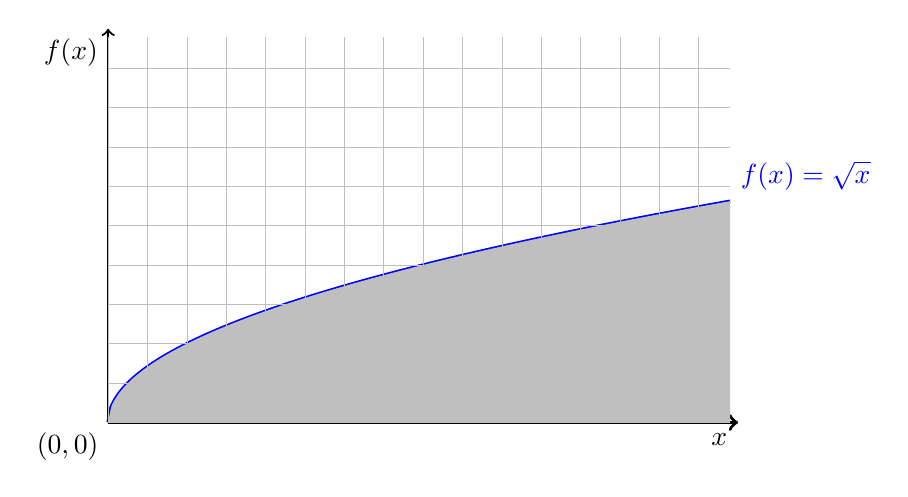
\begin{tikzpicture}
		\draw (0,0)--(0,0) node[anchor = north east]{\((0,0)\)};
		\draw[black,thick,->] (0,0) -- (0,5) node[anchor = north east] {\(f(x)\)};
		\draw[black,very thick,->] (0,0) -- (8,0) node[anchor = north east] {\(x\)};
		\draw[blue,very thick,smooth,samples=300,domain=0:7.9] plot(\x,{sqrt(\x)}) node[anchor = south west] {\(f(x)=\sqrt{x}\)};
		\fill[lightgray,smooth,samples=200,domain=0:7.9, variable = \x] (0,0) -- plot(\x,{sqrt(\x)}) -- (7.9,0) -- cycle; 
		\draw[step=0.5cm,lightgray, very thin] (0,0) grid (7.9,4.9); 
	\end{tikzpicture}
	\caption{The subgraph of \(f: \SR^+ \to \SR^+\), \(x\mapsto \sqrt{x}\) is shaded in gray. }%
	\label{fig:subgraph}
\end{figure}

